\begin{comment}
    \begin{mimargen}{-0.65cm}{-1cm}
    \chapter{Entrenamiento}

    Para comenzar con Arduino+TensorFlow, instalaré la bibliotecas
    necesarias para usar TensorFlow y la \textit{Nano 33 Sense}:
    \begin{enumerate}
        \item \textbf{Arduino\_TensorFlowLite}: Permite construir aplicaciones con
        aplicaciones para AI/ML.
        \item \textbf{Arduino\_LSM9DS1}: Provee de las herramientas para acceder al
        acelerómetro, magnetometro y giroscopop del \textit{Nano 33 BLE Sense}.
    \end{enumerate}

    \cite{github-magicwand}Además, hay que realizar una serie de cambios en la biblioteca
    \small\textbf{LSM9DS1.cpp}.\normalsize\\
    Añadir justo antes de que la función \small\textbf{LSM9DS1Class::begin()}\normalsize
    ~retorne:
    \begin{lstlisting}
        // Enable FIFO (see docs https://www.st.com/resource/en/datasheet/DM00103319.pdf)
        writeRegister(LSM9DS1_ADDRESS, 0x23, 0x02);
        // Set continuous mode
        writeRegister(LSM9DS1_ADDRESS, 0x2E, 0xC0);
    \end{lstlisting}

    También debemos editar \small\textbf{LSM9DS1Class::accelerationAvailable()}
    \normalsize:
    \begin{lstlisting}
        int LSM9DS1Class::accelerationAvailable()
        {
            /********************************** OLD *********************************
            if (readRegister(LSM9DS1_ADDRESS, LSM9DS1_STATUS_REG) & 0x01) { 
                return 1; 
            }
            *********************************** OLD *********************************/
        
            // Read FIFO_SRC. If any of the rightmost 8 bits have a value, there is data
            if (readRegister(LSM9DS1_ADDRESS, 0x2F) & 63) {
                return 1;
            }
            
            return 0;
        }
    \end{lstlisting}


    Cuando ya tenemos la biblioteca para los sensores y el acceso al puerto garantizado,
    podemos pasar a probar el programa.
    Si funciona con el entrenamiento por defecto, continuamos finalmente con nuestro
    entrenamiento.\\
    Realizaremos el entrenamiento recogiendo muestras para cada caracter a
    reconocer. Una vez tenemos suficientes muestras para todos los caracteres, podemos
    realizar el entrenamiento del modelo, que realizaremos en \textit{Google Colab}.
    El script de entrenamiento es el siguiente: [\textbf{METER ENLACE}].

    ~\\
    Toma de muestras, para el software que utilizaremos para tomar los datos
    para crear el dataset con el que entrenar el modelo, necesitaremos instalar las
    siguientes bibliotecas:\\
    \cite{apds9960} Arduino\_APDS9960: para disponer de librerías para algunos sensores adicionales.\\
    \cite{cmsisdsp} Arduino\_CMSIS\-DSP: para disponer de arm\_math.h.\\
    \cite{lps22hb} Arduino\_LPS22HB: herramientas para disponer del sensor de presión.\\
    \cite{hts221} Arduino\_HTS221: herramientas para el sensor de temperatura y humedad.


    \subsection{Si la placa deja de ser detectada}
    En la primera subida del programa con los datos de entrenamiento
    creados por mí, la placa dejó de ser detectada por el ordenador.\\
    Lo cual me llevó a pensar que el bootloader se había corrompido.
    Sin embargo, buscando posibles causas, encontré una solución:
    restaurar manualmente la placa, cosa que solo funciona, evidentemente,
    si el bootloader no está dañado.
    Pulsando el botón reset de la placa rápidamente varias veces justo
    al conectarlo al ordenador, puede restaurarse la placa. Si ha funcionado,
    el "L" led se encenderá.
    
    Esto ocurría al incorporar el modelo de datos que yo mismo entrenaba
    y fue uno de los problemas que más tiempo me llevó solucionar, sobre
    todo porque no tenía ningún tipo de referencia de por qué no estaba
    respondiendo correctamente el programa con el nuevo modelo.\\
    Por suerte llegué a la solución:\\~\\
    
    
    \subsection{El modelo de datos entrenado no responde\textsuperscript{\cite{intro-tensor-micro}}}
    Como explico en caso anterior, la incorporar el modelo de datos
    entrenado con el dataset de ejemplo que proporciona TensorFlow,
    al subir el programa a la placa, esta dejaba de reconocerse por
    el ordenador, teniendo que resetear la flash de la placa.
    
    Esto se debía a que el proyecto Arduino no soportaba una de las
    operaciones que realizaba la red neuronal en ese momento: reshape.
    Podemos solucionar esto de dos formas:
    \begin{enumerate}
        \item (No probada) Simplemente hacer uso de \textit{AllOpsResolver},
        de forma que el interprete tendrá acceso a todas las micro-operaciones
        disponibles.
        \item Esta segunda es la más sofisticada, ya que al no disponer
        de todas las operaciones para el interprete, reduciremos la cantidad
        de memoria que ocupamos.\\Es la que yo implementé.
    \end{enumerate}
    
    Añadir la siguiente línea al archivo \small\textbf{*.ino}\normalsize~
    de nuestro proyecto:
    \begin{lstlisting}
    micro_mutable_op_resolver.AddBuiltin(tflite::BuiltinOperator_RESHAPE,
                                          tflite::ops::micro::Register_RESHAPE());
    \end{lstlisting}
    
    De esta forma estamos añadiendo la operación al repertorio de las que tendrá
    disponibles el interprete \small\textit{(static\_interpreter)}\normalsize,
    \small\textbf{micro\_mutable\_op\_resolver}\normalsize.
    
    \begin{figure}[h]
    \begin{lstlisting}[firstnumber=72]
    static tflite::MicroMutableOpResolver micro_mutable_op_resolver;
    micro_mutable_op_resolver.AddBuiltin(
        tflite::BuiltinOperator_DEPTHWISE_CONV_2D,
        tflite::ops::micro::Register_DEPTHWISE_CONV_2D());
    micro_mutable_op_resolver.AddBuiltin(
        tflite::BuiltinOperator_MAX_POOL_2D,
        tflite::ops::micro::Register_MAX_POOL_2D());
    micro_mutable_op_resolver.AddBuiltin(tflite::BuiltinOperator_CONV_2D,
                                         tflite::ops::micro::Register_CONV_2D());
    micro_mutable_op_resolver.AddBuiltin(
        tflite::BuiltinOperator_FULLY_CONNECTED,
        tflite::ops::micro::Register_FULLY_CONNECTED());
    micro_mutable_op_resolver.AddBuiltin(tflite::BuiltinOperator_SOFTMAX,
                                         tflite::ops::micro::Register_SOFTMAX());
    micro_mutable_op_resolver.AddBuiltin(tflite::BuiltinOperator_RESHAPE,
                                         tflite::ops::micro::Register_RESHAPE());
    \end{lstlisting}
    \caption{Fragmento de \small\textbf{*.ino}\normalsize~ de nuestro proyecto.}
    \end{figure}
    
    Este fragmento de código ilustra lo que acabo de explicar.
    
    
    \subsection{Error durante el entrenamiento}
    Al comenzar con mi primer pequeño dataset para comprobar cuán realizable es
    mi idea para este modelo, tuve un error que me tuvo durante un buen tiempo
    ocupado.
    
    \begin{figure}[h]
        \centering
        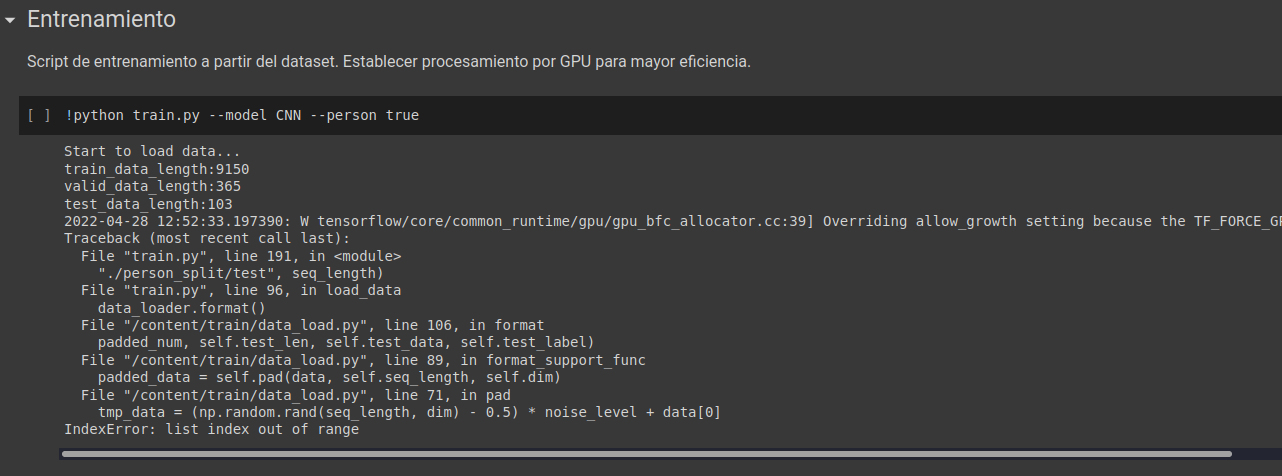
\includegraphics[width=1\textwidth]{capturas/ErrorEntrenamiento.png}\\[-0,40cm]
        \caption{Error durante primer entrenamiento con un dataset propio.}
        \end{figure}
    
    Tras revisar que no se debía a la longitud de las secuencias de datos,
    como hace pensar el mensaje de error, fui a intentar reducir el tamaño de las
    muestras del dataset y fue cuando vi que había un error en una de las muestras,
    de forma que había un separador (' -,-,-') sin información.\\
    Al eliminarlo, el entrenamiento ya no arrojaba errores.
    
    
    \subsection{Error al cambiar el tamaño de las secuencias de movimientos}
    Los movimientos que se deben registrar para las letras son, en general, más complejos
    que los que incluye el dataset de ejemplo. Por lo tanto las secuencias de registro
    de movimiento, serán mayores. Esto supone un problema porque el modelo está ajustado
    al dataset de ejemplo y por tanto, se queda algo corto para nuestro propósito.
    El error se da al cambiar el tamaño de dicha secuencia
    (\small\textbf{seq\_length}\normalsize) en \small\textbf{train.py}\normalsize~ y
    \small\textbf{train\_test.py}\normalsize~.
    
    \begin{figure}[h]
        \centering
        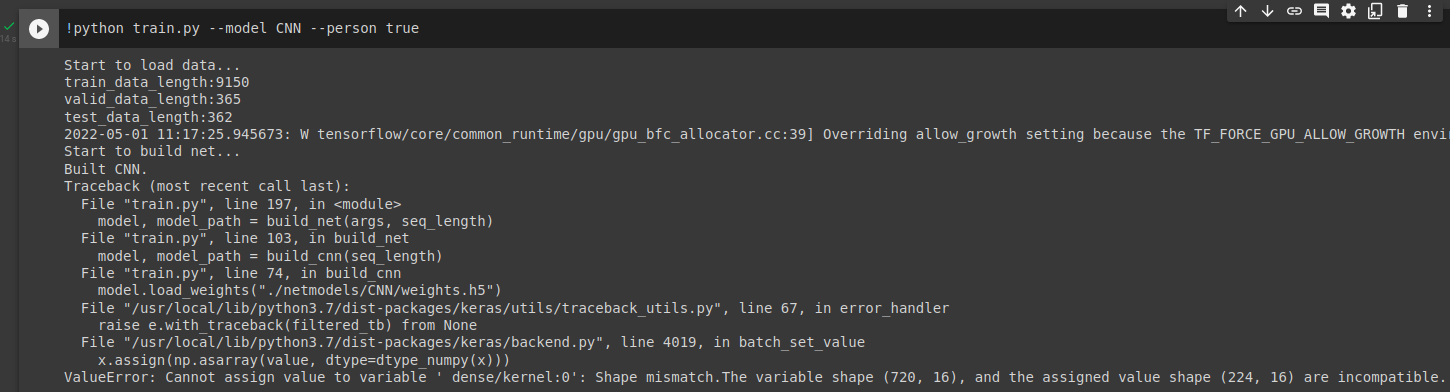
\includegraphics[width=1\textwidth]{capturas/ErrorTamanioSecuencias.png}\\[-0,40cm]
        \caption{Error al cambiar el tamaño de secuencia de movimientos.}
        \end{figure}
    
    Tras mucha documentación sobre Tensorflow, y no obtener la causa del error; pensé
    que esto ya me pasó por culpa de la configuración del \small\textbf{*.ino}\normalsize~.
    Así que fui a revisarlo y efectivamente, hay un parámetro en este archivo sujeto a
    la longitud de los datos. Tras cambiarlo, funcionaba correctamente de nuevo, aunque
    sin detectar la letra que estaba probando en el nuevo dataset.

    %\begin{mimargen}{-1cm}{-1cm}

    \chapter{Segundo acercamiento}
    Visto cómo toma pete los datos, pruebo a hacerlo.
    Cargar el programa de recolección de datos en la placa(creo que funciona el magic\_wand,
    PROBAR).
    Acceder a la web de recolección. Recolectar.
    Para acceder a la web, hay que hacerlo con chrome y con la flag
    'Experimental Web Platform features' activa en 'chrome://flags/'


    Hay un error con el DataCollector, además de que asigna mal los índices(index)
    al borrar muestras, no guarda todas las muestras que tomas, da la sensación de que
    hay un límite.
    Para contar el número de muestras que hay en el JSON, uso la siguiente línea bash:
    \begin{lstlisting}[language=bash]
    ~$ grep -o index <nombre_archivo>.json | wc -l
    \end{lstlisting}

    \textbf{LA OBTENCIÓN DE DATOS TIENE UN FALLO AL BORRAR MUESTRAS} \\
    Este fallo aparentemente se produce al borrar instancias por debajo de
    la última. En ocasiones, se produce un pequeño error en las comprobaciones
    de índices de muestras, por lo que se borran varias muestras y estas terminan
    con índices desordenados.\\
    Para paliar este problema y comprobar si había el número de trazos esperado,
    se hacía uso de un comando en bash cada vez que se generara un \textit{JSON}:
    grep -o -i index ./wanddata.json | wc -l

    \textbf{MODELO}\\
    Se trata de un modelo de aprendizaje supervisado, es decir, que está basado en
    etiquetas(\textit{labels}) estas etiquetas representarán las distintas soluciones
    a las que hará frente el modelo; en nuestro caso, letras.
    La forma que emplearemos para representar dichas letras como input para el modelo,
    serán imágenes. Aunque para tomar dichas imágenes, hacemos uso del giroscopio
    y el acelerómetro de la placa.\\


    \textbf{LEER DEL PUERTO SERIE EN QT}
    Hay que añadir al *.pro del proyecto QT:
    \begin{lstlisting}[language=make]
    QT += serialport
    \end{lstlisting}
    Y tras esto, añadir la biblioteca con normalidad y acceder al puerto
    con el nombre, en nuestro caso, "ttyACM0".

    \textbf{FALLO RECONOCIMIENTO DE IMÁGENES QT}\\
    Al importar imágenes en QT tras haber exportado el programa a Win y Linux para
    probar que todo fuera correctamente, las imágenes dejaron de mostrarse.\\
    Esto se debe a que cambió la ruta del proyecto al directorio en el que se
    exportó. Por tanto las rutas especificadas para las imágenes, dejaron de ser
    válidas. Para corregir este problema, basta con cambiar el 'Build directory' del
    proyecto(Desde 'Projects' en el panel de la derecha del QT creator).\\

    \textbf{HEBRAS QT}\\
    Para la lectura del puerto serie desde el programa, necesitamos imporat

    \textbf{VISOR WEB QT}\\
    Para hacer empotrar html en qt, importamos las bibliotecas de QWeb. Para ello,
    necesitamos aantes instlar todo el QtWebKit siguiendo las instrucciones:
    \url{https://github.com/OpenBoard-org/OpenBoard/wiki/Build-OpenBoard-on-Ubuntu-20.04}

    \textbf{VINCULAR PUERTO SERIE A PLACA}\\
    Para ello, haré uso de las reglas de udev del sistema linux.
    Lo primero es conocer la información de nuestra placa:
    \begin{lstlisting}[language=make]
    ~$ lsusb
    [...]
    Bus 003 Device 004: ID 2341:805a Arduino SA Nano 33 BLE
    [...]
    \end{lstlisting}
    De aquí podemos extraer el fabricante(o idVendor) y el producto de este fabricante
    (o idProduct). Necesitaremos ambos.

    Ahora necesitamos el serial del puerto al que vincularemos la placa:
    \begin{lstlisting}[language=make]
    ~$ udevadm info -a -n /dev/ttyACM0 | grep serial
    ATTRS{serial}=="185F25FD3EF48040"
    \end{lstlisting}
    Con esto, ya podemos crear la regla para vincular univocamente el puerto a la placa
    y evitar así problemas con la detección en el UI.\\
    En /etc/udev/rules.d/99-ftdi.rules (en mi caso, varía dependiendo del sistema),
    crearemos la regla \\SUBSYSTEM=="tty", ATTRS{idVendor}=="2341", ATTRS{idProduct}=="805a",
    ATTRS{serial}=="185F25FD3EF48040", SYMLINK+="ttySLAB0"\\por los datos obtenidos.\\

    \textbf{CAMBIOS MODELO}\\
    Cambiar el tamaño del kernel de las capas Conv2D de 3 a 4, resulta muy efectivo,
    a costa, evidentemente, de aumentar el tamaño que ocupa el modelo.\\
    Al pasar de 4 a 5, el modelo arroja unos datos de efectividad teóricos extremadamente
    buenos, alcanzando cifras de precisión mucho más altas con menos epochs.
    En general, podemos extrapolar que, a mayor tamaño del kernel, mejor precisión pero
    mayor tamaño del modelo. En nuestro caso no llega a ser un problema, ya que, aunque
    estamos usando un dispositivo de memoria limitada, no llega a ocuparse toda la memoria
    del mismo, al menos por ahora.\\

    \textbf{PRUEBAS BLUETOOTH}\\
    He tenido que instalar qtconnectivity5-dev para probar el QT project que estoy probando.\\

    \textbf{POR QUÉ ESTA PLACA?}\\
    Aduino Nano Sense 33 BLE\\
    Por qué arduino: Documentación, respaldo comunidad, IDE facilita trabajo, etc.\\
    Por qué Nano: Queremos integrarla en un 'lápiz', debe ser un dispositivo pequeño.\\
    Por qué Sense: Necesitamos los sensores para el reconocimiento de movimiento.\\
    BLE: Por pura utilidad, es mucho más cómodo utilizar el lápiz de forma inalámbrica.
    Además no tiene mucho sentido integrar el procesamiento en un dispositivo pequeño
    si va a depender de un ordenador.\\

    \textbf{DESCONEXIÓN DEL PROGRAMA A BT AL ESCRIBIR PLACA EN RX}\\
    Para el control de flujo de la comunicación bluetooth(asegurarse de que recibimos
    bien y solo una vez cada letra), implemento un sistema de señales.
    Cuando recibimos una letra desde la placa(mediante canal tx), el programa la almacena y
    envía una señal de que ha recibido la letra(mediante canal rx) y cuando la placa
    recibe esta señal, borra del canal tx la letra para que no vuelva a leerse desde el
    programa.


    \textbf{PROBLEMAS UI-BLUETOOTH}\\
    Desconexiones random cada cierto tiempo durante lectura BLE.
    Lecturas dobles al escribir durante reconexión.

    \textbf{BUFFER PARA SINCRONIZACIÓN DE ESCRITURA AUTÓNOMA}\\

    \textbf{MÉTODO DE ENVÍO DE BUFFER DE LETRAS PARA CONEXIÓN BT CUANDO HAYA UNA CADENA
    PREVIA A CONEXIÓN}\\




    %\end{mimargen}

    \end{mimargen}
\end{comment}